\myparagraph{Purpose}
One of the great feature of \textit{Track4Run} is the possibility for a runner to be able to enrol in a \textit{Run}.
In order to enrol in a \textit{Run} a runner must be logged in \textit{Track4Run} application, he/she has to search the \textit{Run} that he/she wants in the \textit{Enrol in a Run} section and finally enrols in it.
However, the \textit{Run} could be already done or the enrolling time expired.

\myparagraph{Scenario 1}
Andrea is a technological boy. A few weeks ago he found in the Play Store the new app \textit{Track4Run} and shared his discovery with his friends. Yesterday, while he was hanging out with the buddies they discovered a new run for the week-end after.
So, Andrea took his phone, opened \textit{Track4Run} app, logged in, clicked on the "\textit{Enrol in a Run}" button and found it on the top of the page. So Andrea clicked on it and when the \textit{Run} event was opened he cliked on the "\textit{Enrol}" button.
After that Andrea received a confirmation e-mail about the correctness of the enrolment.

\myparagraph{Scenario 2}
Samanta loves walking but for a few months now she started running. She spoke about the city \textit{Run} planned in two days with her friend Federica, but unfortunately when she took her phone and opened \textit{Track4Run} she discovered that the time to enrol in the \textit{Run} was expired yet.

\myparagraph{Use Case}
The \textit{Enrol In A Run} use case is analyzed in Table \ref{table:enrolRunTable}.

\myparagraph{Mockup}
The \textit{Enrol In A Run} mockup is shown in Figure \ref{img:enrolInARunMockup}.

\myparagraph{Functional requirements}
\begin{enumerate}
  \item The system must not accept an enrolment in a \textit{Run} where a \textbf{Runner} is enrolled yet.
  \item The system must not accept an enrolment in a \textit{Run} where the enrolment time is expired yet.
  \item The system must not accept an enrolment in a \textit{Run} where the maximum number of enrolments is reached;
  \item The system must not accept an enrolment in a \textit{Run} where a \textbf{Runner} and the \textit{Organizer} are the same person.
  \item The system must let the \textbf{Runner} leave the enrolment process at anytime.
\end{enumerate}

\begin{center}
\begin{table}
\begin{tabular}{ | l | p{0.75\linewidth} | }
  \hline
    Actor & \textbf{Runner} \\ \hline
    Goal & \textbf{[G.12]} \\ \hline
    Input Condition & The \textbf{Runner} wants to enrol in a \textit{Run} \\ \hline
    Event Flow & \begin{minipage}[t]{0.7\textwidth}
      \begin{enumerate}
        \item The \textbf{Runner} opens \textit{Track4Run} service through mobile application and he/she logs in;
        \item The \textbf{Runner} clicks on "\textit{Enrol in a Run}" button;
        \item The \textbf{Runner} looks for a \textit{Run} through the search bar or looking to the proposed ones;
        \item The \textbf{Runner} clicks on the \textit{Run} he/she wants to enrol in;
        \item The \textbf{Runner} clicks on the "\textit{Enrol}" button.
      \end{enumerate}
    \smallskip
  \end{minipage} \\ \hline
  Output Condition & The system registers the enrolment of the \textbf{Runner} and it notifies him/her with a confirmation e-mail. \\ \hline
  Exceptions & \begin{minipage}[t]{0.7\textwidth}
    \begin{itemize}
      \smallskip
      \item If functional requirements 1, 2, 3 or 4 are not satisfied the system notifies the \textbf{Runner} with an error message and the process goes back to step 3;
      \item If the \textbf{Runner} looks for a \textit{Run} that is not present in the system, the system notifies him/her with a warning message;
      \item If the \textbf{Runner} decides to leave the enrolment process this one is aborted.
    \end{itemize}
    \smallskip
  \end{minipage}  \\ \hline
\end{tabular}
\caption{\textit{Enrol In A Run} use case}
\label{table:enrolRunTable}
\end{table}
\end{center}

\begin{figure}
\begin{center}
  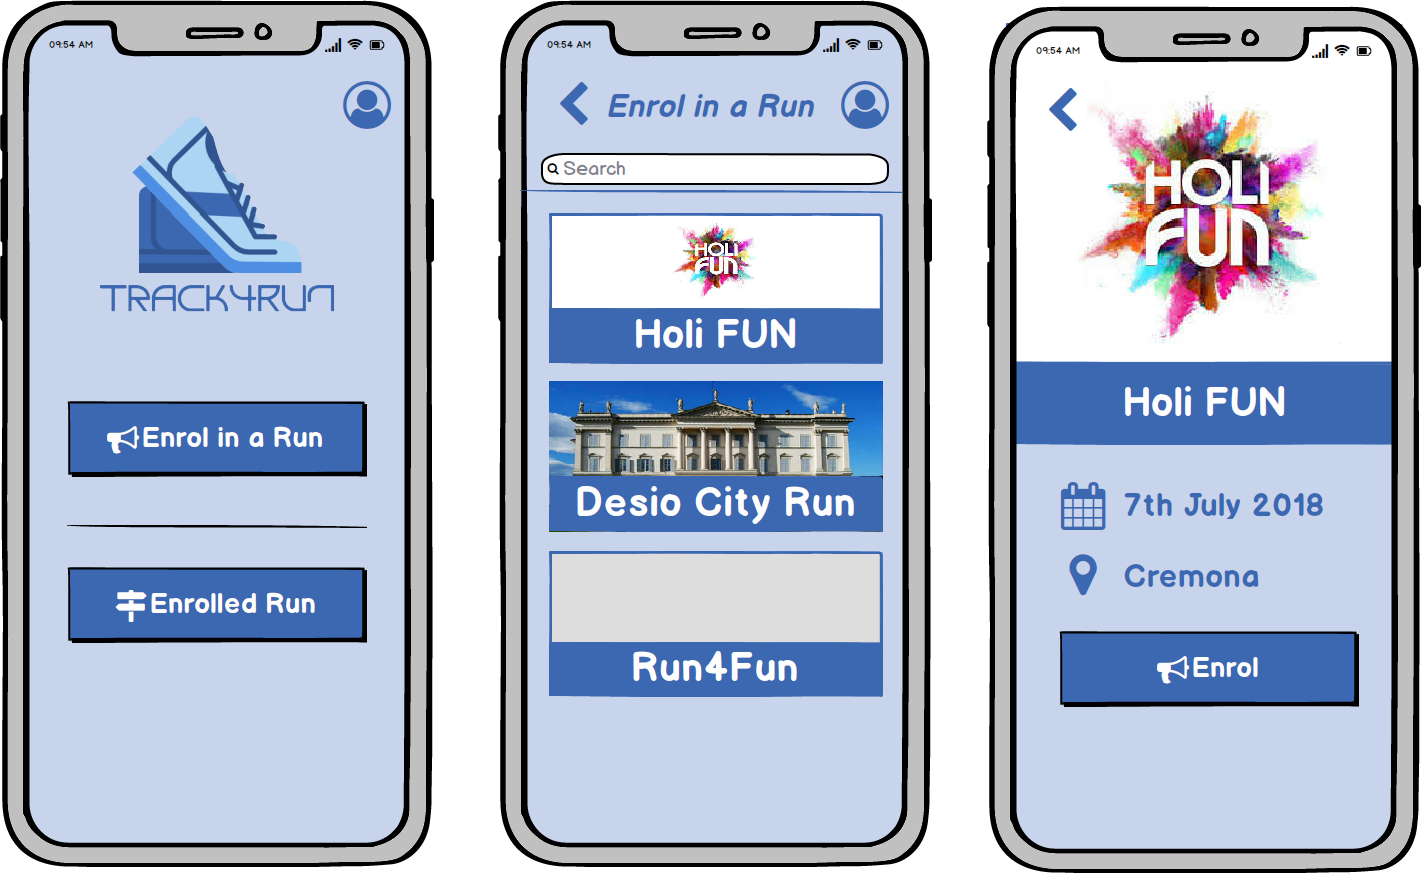
\includegraphics[width=\textwidth]{img/mockup/EnrolRun.png}
  \hspace{0.05\linewidth}
  \centering
  \caption{\textit{Enrol In A Run} mockup}
  \label{img:enrolInARunMockup}
\end{center}
\end{figure}
